\section{Centered-square results}
\label{app:square}

\begin{table}[h]
\centering
\caption{Parameter-wise centered-square routing and T2-C results at $K=24$. The mean weight is the steady weight for $S$--$H$ and the periodic weight for $H$--$P$.}
\label{tab:square_parameter}
\small
\setlength{\tabcolsep}{3.5pt}
\begin{tabular}{lrlrrrr}
\toprule
Overlap & $Re$ & E2 choice & $\bar\alpha$ & E2 joint & T2-C joint & reduction \\
\midrule
$S$--$H$ & 95.1 & Hopf & 0.0967 & 1.7140 & 1.1827 & 31.00\% \\
$S$--$H$ & 95.3 & Hopf & 0.0971 & 1.7456 & 1.2090 & 30.74\% \\
$H$--$P$ & 100.5 & Hopf & 0.5870 & 2.6485 & 0.8571 & 67.64\% \\
$H$--$P$ & 102.0 & Periodic & 0.7094 & 1.0462 & 0.8360 & 20.09\% \\
\bottomrule
\end{tabular}
\end{table}

The aggregate local-specialist errors are $(E_u,E_p)=(1.5311,1.4583)\%$ for steady flow, $(0.4387,0.4844)\%$ for Hopf-onset flow, and $(0.9395,1.0921)\%$ for periodic flow. On the aggregate $S$--$H$ evaluation, the steady and Hopf specialists have joint errors $4.8426\%$ and $1.7298\%$; on $H$--$P$, the periodic and Hopf specialists give $1.2079\%$ and $2.8718\%$. These results show why the best local choice can change between overlaps and why a corrected convex assembly is useful.

Figures~\ref{fig:app_square_sh_full} and \ref{fig:app_square_hp_full}
provide the complete velocity, gauge-corrected pressure, and pointwise-error
views underlying the compact main-text comparison.

\begin{figure}[p]
\centering
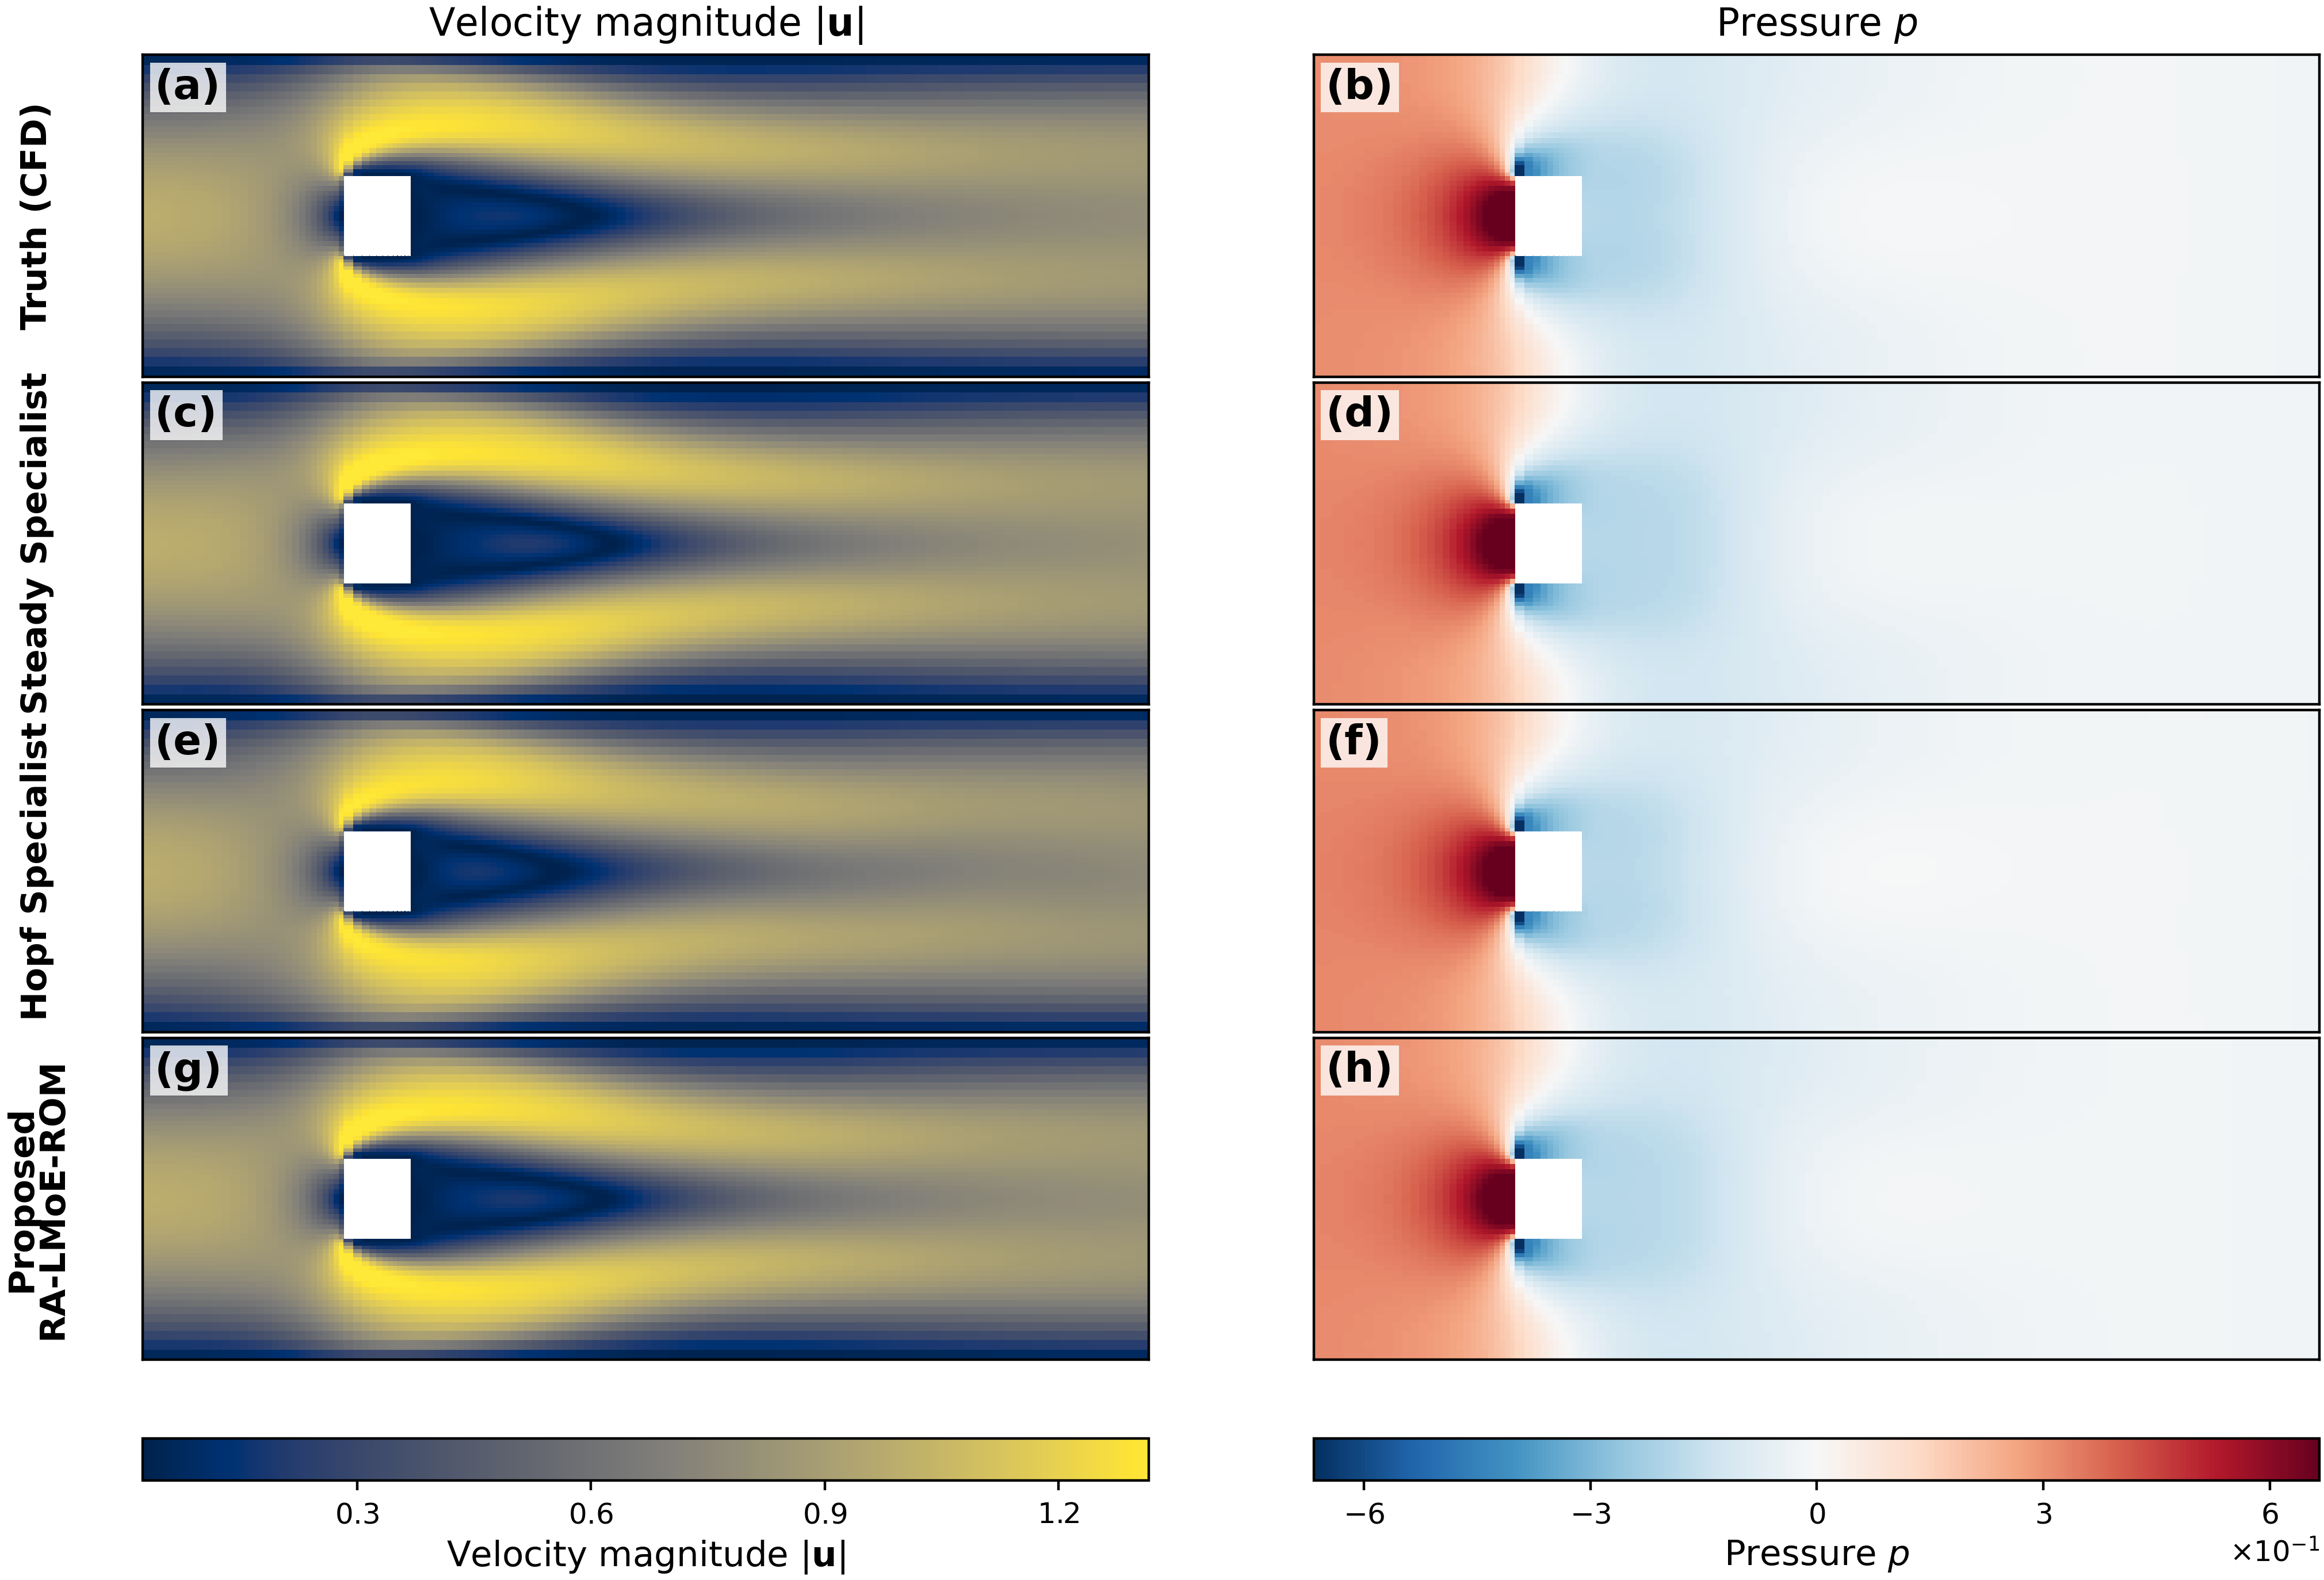
\includegraphics[width=0.80\linewidth]{figures/original/SH_2.png}

\vspace{0.35em}
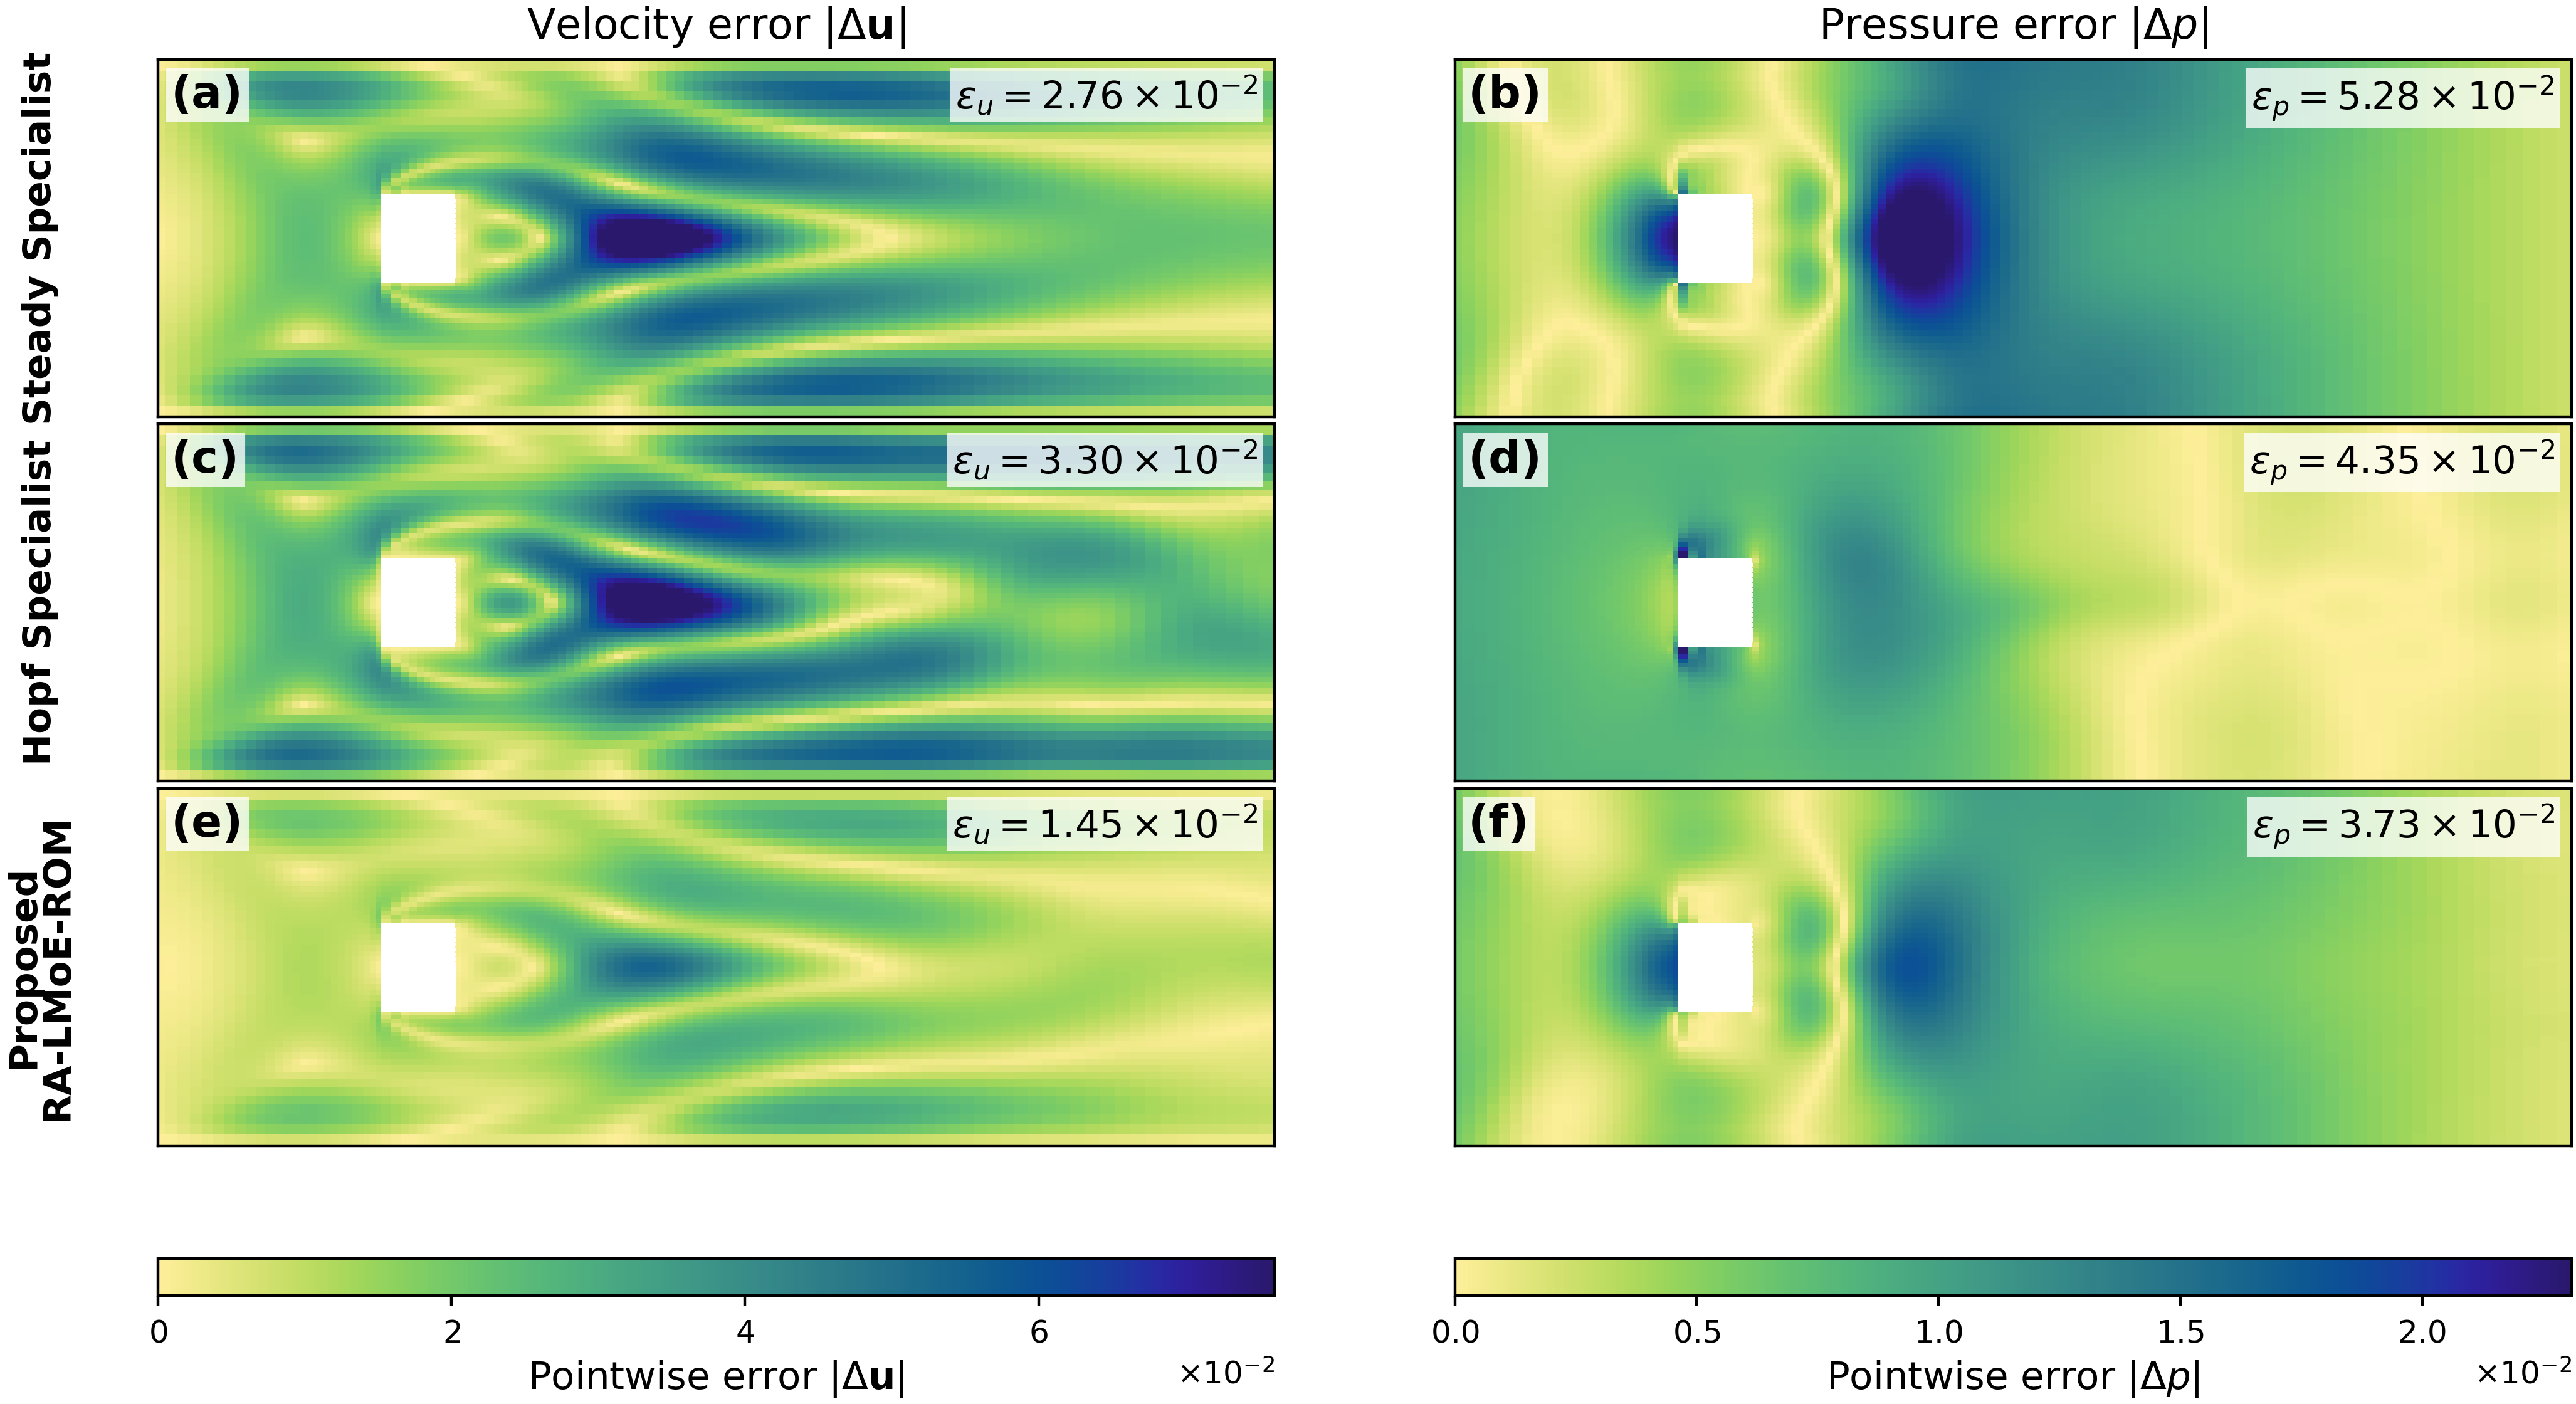
\includegraphics[width=0.80\linewidth]{figures/original/SH_2_1.png}
\caption{Representative held-out prediction in the centered-square
$S$--$H$ overlap at $Re=95.1$. The upper panel compares the CFD reference,
Steady specialist, Hopf specialist, and T2-C prediction for velocity
magnitude and gauge-corrected pressure. The lower panel gives the
corresponding pointwise absolute errors.}
\label{fig:app_square_sh_full}
\end{figure}

\begin{figure}[p]
\centering
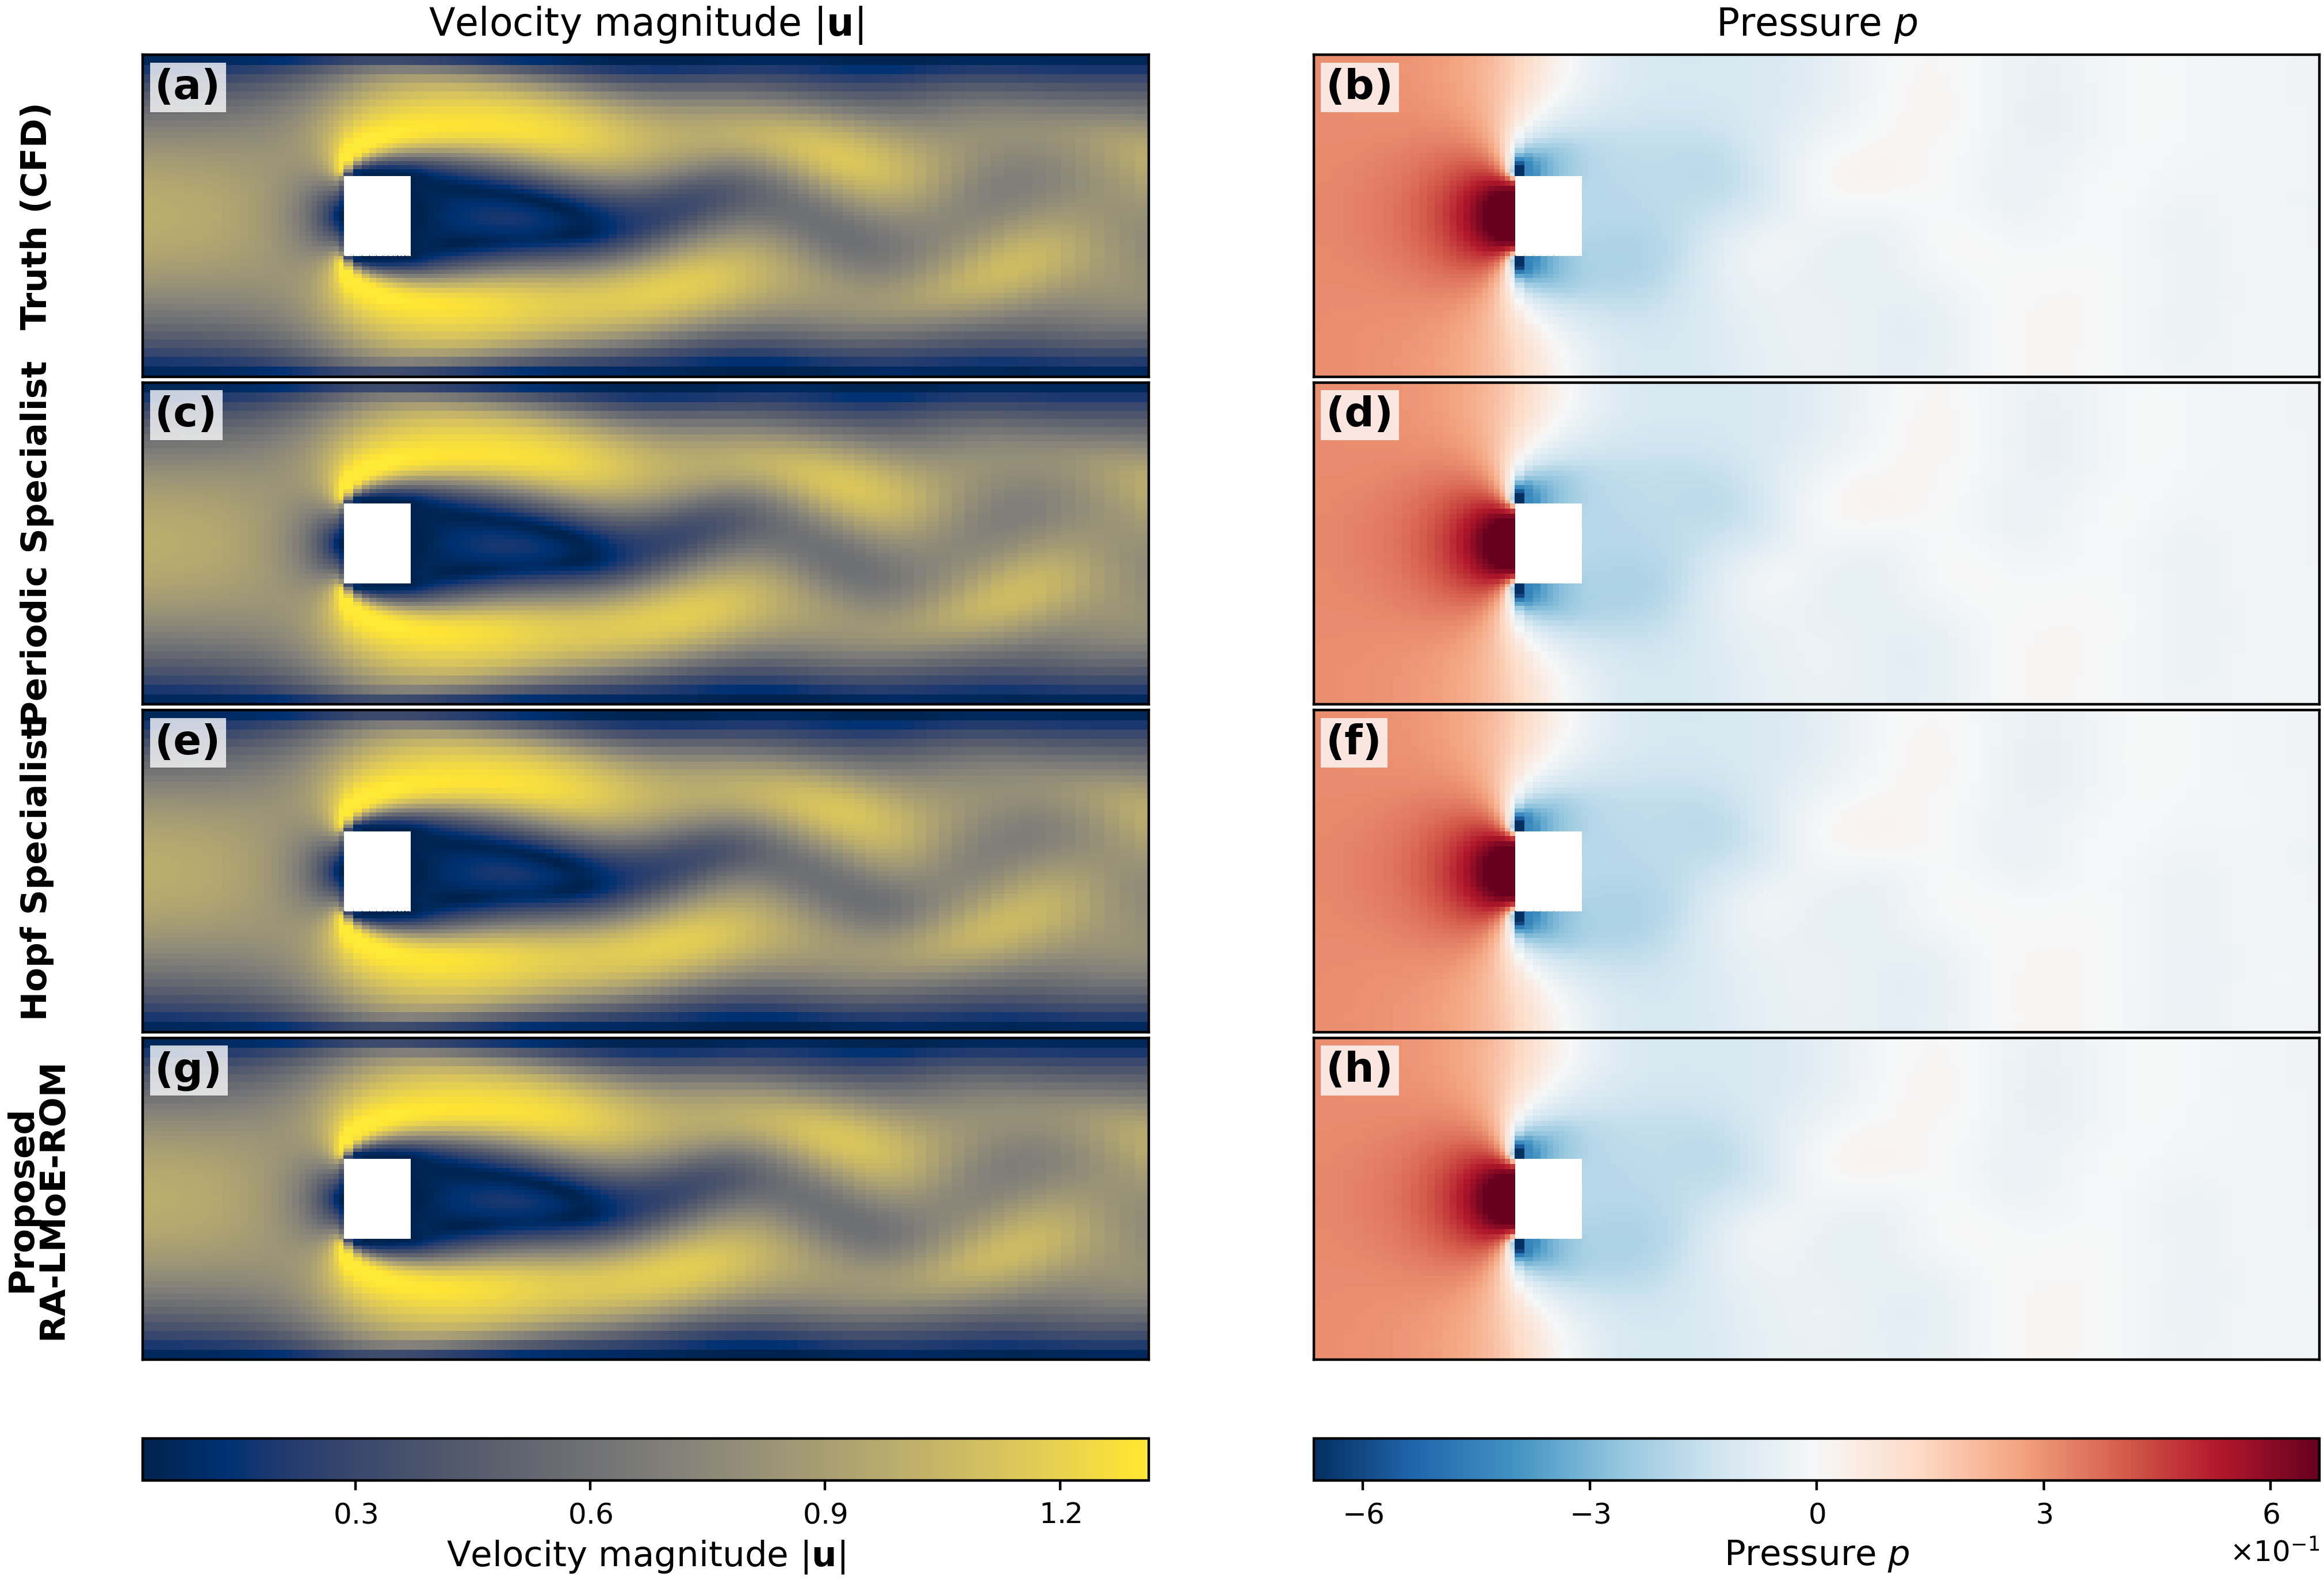
\includegraphics[width=0.80\linewidth]{figures/original/HP_2.png}

\vspace{0.35em}
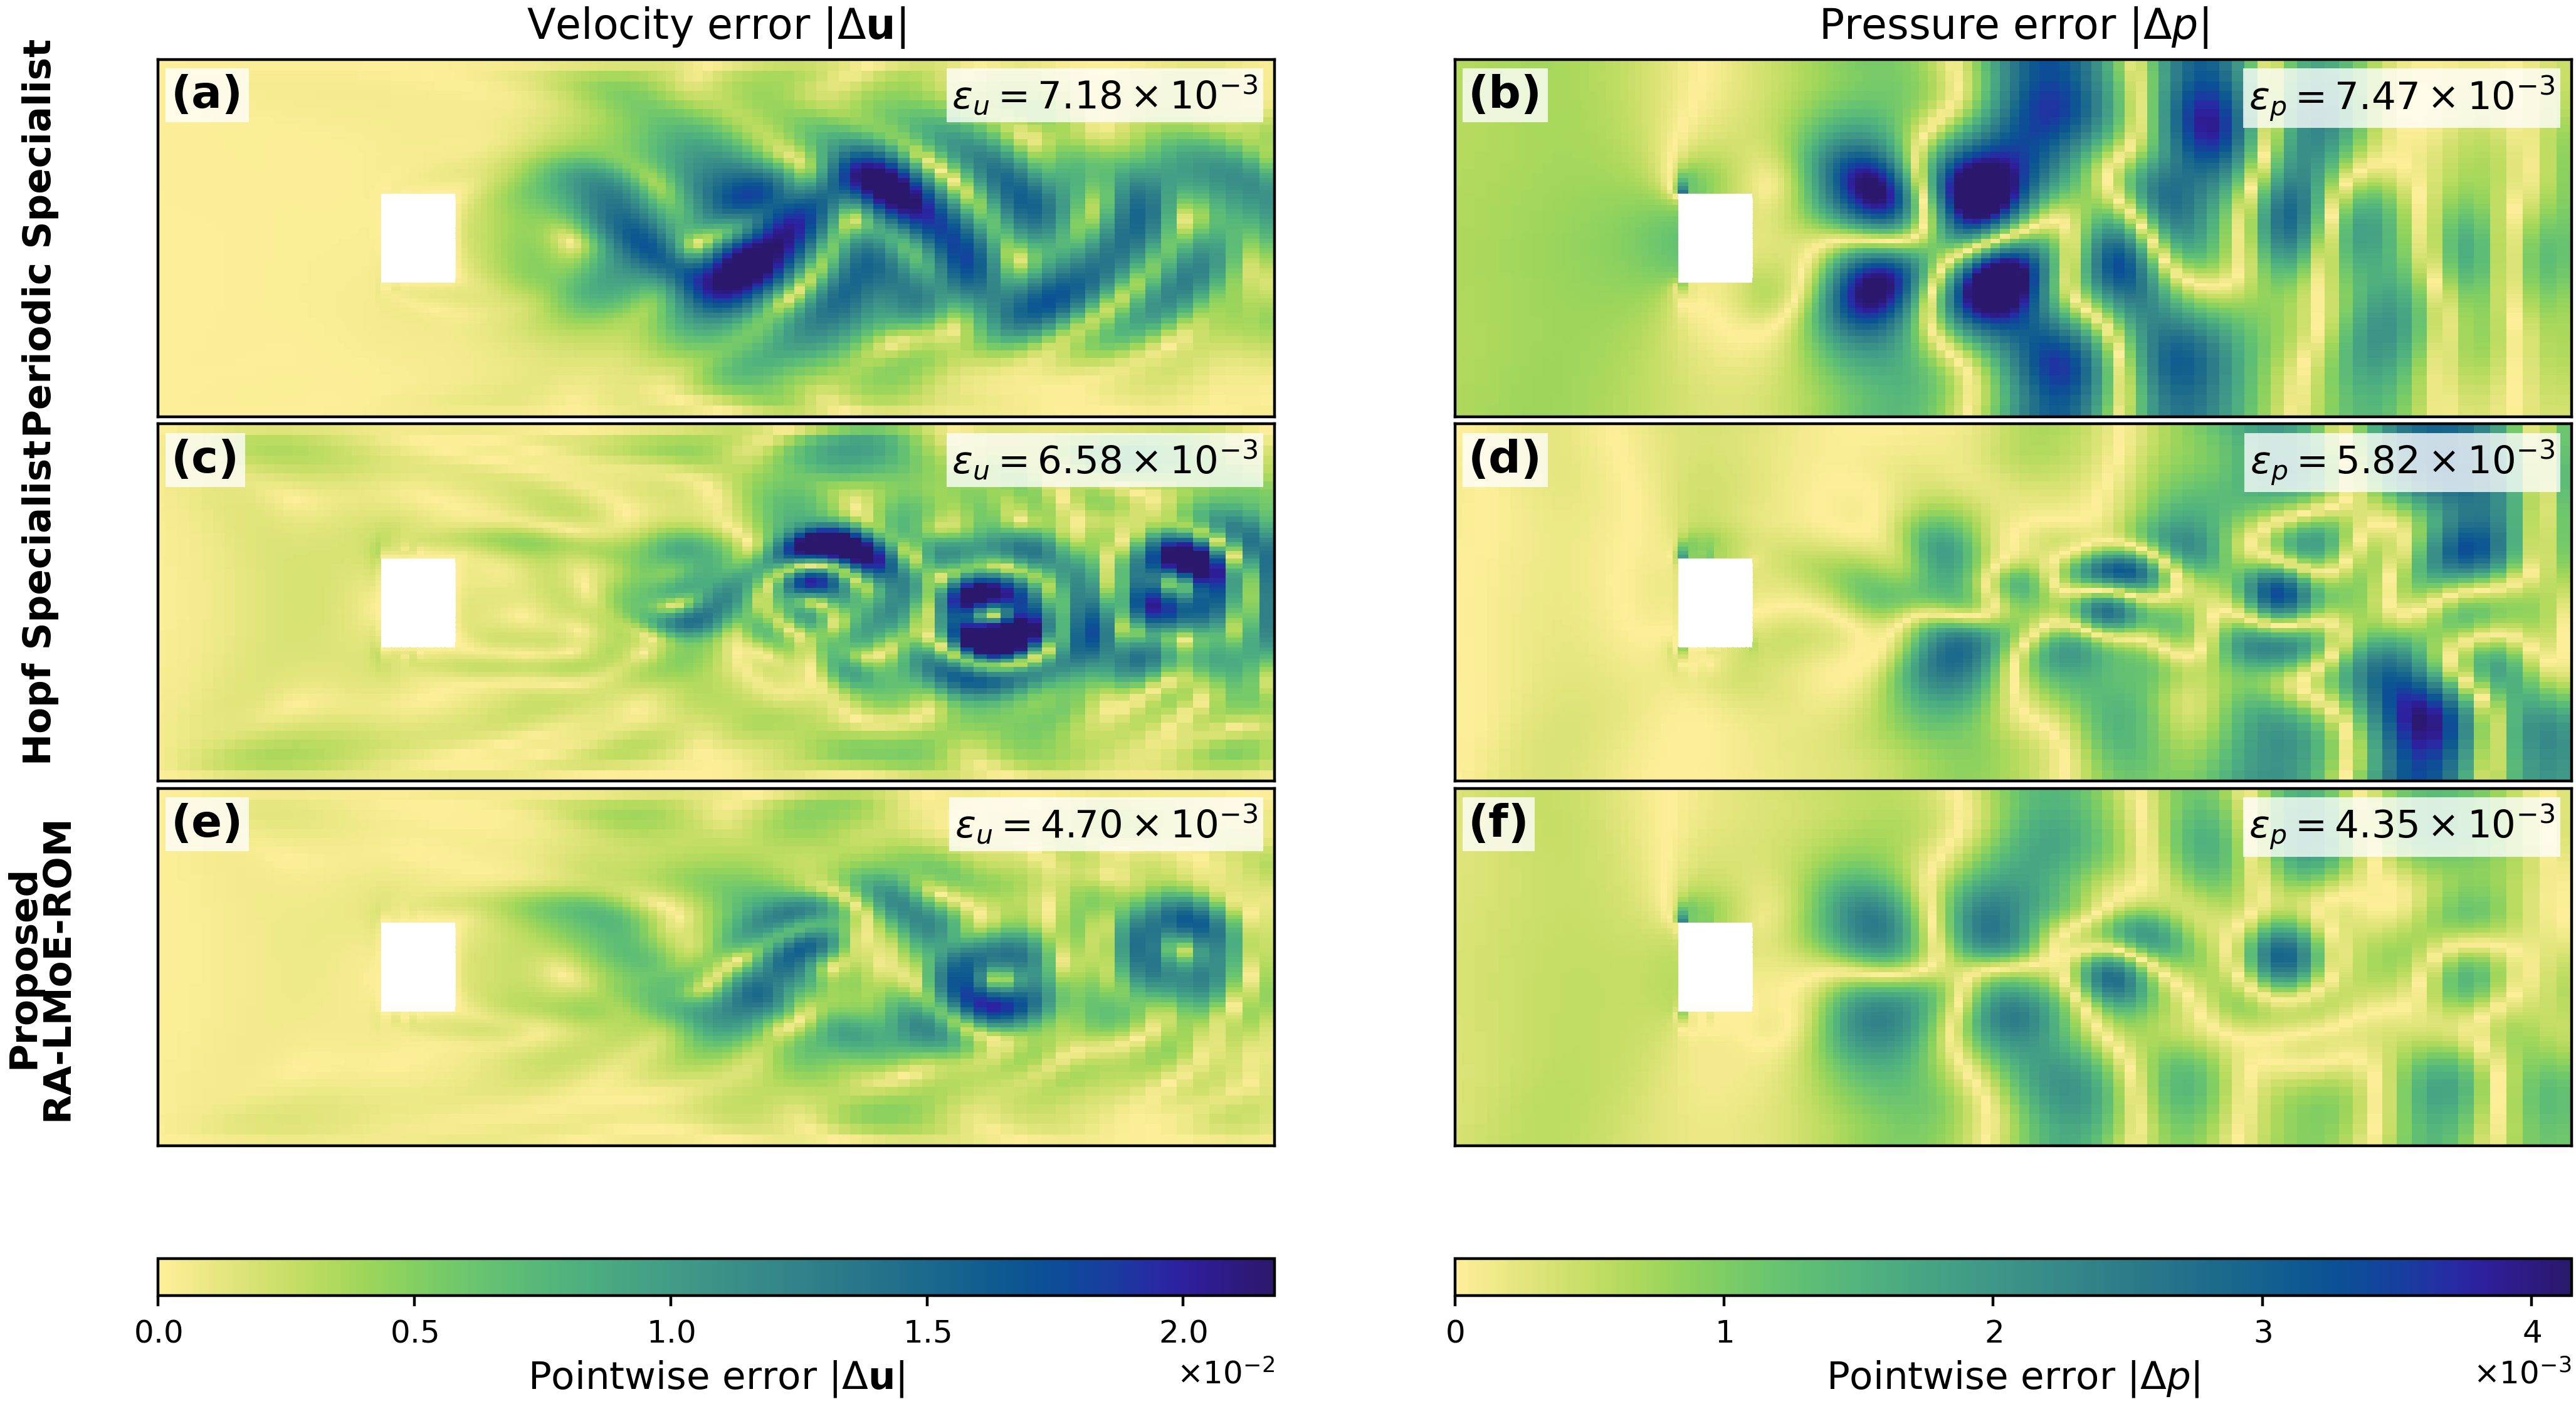
\includegraphics[width=0.80\linewidth]{figures/original/HP_2_1.png}
\caption{Representative held-out prediction in the centered-square
$H$--$P$ overlap at $Re=100.5$. The upper panel compares the CFD reference,
Periodic specialist, Hopf specialist, and T2-C prediction for velocity
magnitude and gauge-corrected pressure. The lower panel gives the
corresponding pointwise absolute errors.}
\label{fig:app_square_hp_full}
\end{figure}
